
\chapter{Results}
\label{chapter:results}

\section{End-to-End Latency}
\label{sec:e2e_latency}

This section presents the end-to-end latency results of the proposed real-time simultaneous interpretation system. Following the evaluation framework defined in Section~\ref{sec:evaluation_framework}, latency is quantified using Average Lagging (AL), Length-Adaptive Average Lagging (LAAL), and Real-Time Factor (RTF). These metrics jointly capture the temporal alignment between source speech and translated output, the effect of output length variability, and the system’s ability to sustain real-time operation. End-to-end latency is a primary indicator of usability in simultaneous interpretation scenarios, as excessive delay directly degrades comprehension, listener comfort, and perceived synchronicity.

\subsection{Baseline Configuration}
\label{subsec:baseline_e2e}

The baseline configuration represents the default system setup defined in the evaluation framework, consisting of Microsoft Azure Streaming Speech-to-Text, DeepL neural machine translation, and Microsoft Azure Text-to-Speech, with all other system parameters held constant.

Table~\ref{tab:baseline_al} reports the AL measured across three independent runs. The results indicate a consistent temporal offset between source speech and translated audio output, with limited variability across repetitions. This suggests stable real-time behavior under the baseline configuration.

\begin{table}[!htbp]
\centering
\caption[Baseline Average Lagging results]{AL results for the baseline configuration across three runs}
\label{tab:baseline_al}
\begin{tabular}{lcccc}
\toprule
\textbf{Metric} & \textbf{Run 1} & \textbf{Run 2} & \textbf{Run 3} & \textbf{Mean $\pm$ Std} \\
\midrule
AL (s) & 2.18 & 2.24 & 2.21 & 2.21 $\pm$ 0.03 \\
\bottomrule
\end{tabular}
\end{table}

To account for potential length mismatches between source and translated output, LAAL was also computed. As shown in Table~\ref{tab:baseline_laal}, LAAL values are slightly higher than standard AL, reflecting normalization for output length variability while maintaining similar run-to-run stability.

\begin{table}[!htbp]
\centering
\caption[Baseline Length-Adaptive Average Lagging results]{LAAL results for the baseline configuration}
\label{tab:baseline_laal}
\begin{tabular}{lcccc}
\toprule
\textbf{Metric} & \textbf{Run 1} & \textbf{Run 2} & \textbf{Run 3} & \textbf{Mean $\pm$ Std} \\
\midrule
LAAL (s) & 2.31 & 2.36 & 2.33 & 2.33 $\pm$ 0.03 \\
\bottomrule
\end{tabular}
\end{table}

The RTF results for the baseline configuration are summarized in Table~\ref{tab:baseline_rtf}. Across all runs, the RTF remains well below unity, indicating that the system processes input audio faster than real time and does not accumulate backlog during continuous operation.

\begin{table}[!htbp]
\centering
\caption[Baseline Real-Time Factor results]{RTF results for the baseline configuration}
\label{tab:baseline_rtf}
\begin{tabular}{lcccc}
\toprule
\textbf{Metric} & \textbf{Run 1} & \textbf{Run 2} & \textbf{Run 3} & \textbf{Mean $\pm$ Std} \\
\midrule
RTF & 0.82 & 0.85 & 0.83 & 0.83 $\pm$ 0.02 \\
\bottomrule
\end{tabular}
\end{table}

Across all runs, the baseline configuration exhibits consistent end-to-end latency behavior with limited run-to-run variance. Average Lagging remains within a narrow range, indicating stable temporal alignment between source speech and translated output. The slightly higher LAAL values reflect the effect of variable translation length, while RTF values below unity confirm that the system is able to sustain real-time operation without cumulative delay buildup.


\subsection{Alternative Configurations}
\label{subsec:alternative_e2e}

To evaluate the robustness of the proposed system architecture, alternative configurations were tested by replacing individual pipeline components while keeping all other parameters identical to the baseline setup described in Section~\ref{subsec:baseline_e2e}. Specifically, the ASR component and the TTS component were swapped independently, while the NMT stage and segmentation logic remained unchanged. This controlled variation allows the impact of individual components on end-to-end latency to be assessed without introducing confounding architectural changes.

Table~\ref{tab:al_all_configs} summarizes the AL results across the baseline and alternative configurations. All configurations exhibit comparable lag values with limited variance across runs, indicating consistent temporal behavior regardless of the selected ASR or TTS provider.

\begin{table}[!htbp]
\centering
\caption[Average Lagging across configurations]{AL results across baseline and alternative configurations}
\label{tab:al_all_configs}
\begin{tabular}{lcccc}
\toprule
\textbf{Configuration} & \textbf{Run 1} & \textbf{Run 2} & \textbf{Run 3} & \textbf{Mean $\pm$ Std} \\
\midrule
Baseline (Azure ASR + Azure TTS) & 2.18 & 2.24 & 2.21 & 2.21 $\pm$ 0.03 \\
Alt-ASR (Google ASR)             & 2.26 & 2.31 & 2.28 & 2.28 $\pm$ 0.03 \\
Alt-TTS (Google TTS)             & 2.20 & 2.27 & 2.23 & 2.23 $\pm$ 0.04 \\
\bottomrule
\end{tabular}
\end{table}

The corresponding LAAL results are reported in Table~\ref{tab:laal_all_configs}. As expected, LAAL values are slightly higher than standard AL due to normalization for output length differences. Nevertheless, the relative ordering and variance patterns across configurations remain consistent, confirming comparable streaming behavior.

\begin{table}[!htbp]
\centering
\caption[Length-Adaptive Average Lagging across configurations]{LAAL results across baseline and alternative configurations}
\label{tab:laal_all_configs}
\begin{tabular}{lcccc}
\toprule
\textbf{Configuration} & \textbf{Run 1} & \textbf{Run 2} & \textbf{Run 3} & \textbf{Mean $\pm$ Std} \\
\midrule
Baseline (Azure ASR + Azure TTS) & 2.31 & 2.36 & 2.33 & 2.33 $\pm$ 0.03 \\
Alt-ASR (Google ASR)             & 2.39 & 2.44 & 2.41 & 2.41 $\pm$ 0.03 \\
Alt-TTS (Google TTS)             & 2.35 & 2.42 & 2.38 & 2.38 $\pm$ 0.04 \\
\bottomrule
\end{tabular}
\end{table}

Table~\ref{tab:rtf_all_configs} presents the RTF results for all configurations. In all cases, RTF remains below unity, indicating that the system sustains real-time processing without backlog accumulation. Minor differences between configurations reflect variations in service response times rather than architectural limitations.

\begin{table}[!htbp]
\centering
\caption[Real-Time Factor across configurations]{RTF results across baseline and alternative configurations}
\label{tab:rtf_all_configs}
\begin{tabular}{lcccc}
\toprule
\textbf{Configuration} & \textbf{Run 1} & \textbf{Run 2} & \textbf{Run 3} & \textbf{Mean $\pm$ Std} \\
\midrule
Baseline (Azure ASR + Azure TTS) & 0.82 & 0.85 & 0.83 & 0.83 $\pm$ 0.02 \\
Alt-ASR (Google ASR)             & 0.87 & 0.89 & 0.88 & 0.88 $\pm$ 0.01 \\
Alt-TTS (Google TTS)             & 0.84 & 0.87 & 0.86 & 0.86 $\pm$ 0.02 \\
\bottomrule
\end{tabular}
\end{table}

Figure~\ref{fig:e2e_latency_comparison} summarizes the mean end-to-end latency metrics across all evaluated configurations, highlighting the consistency of system behavior under component substitution.


\begin{figure}[!htbp]
  \centering
  \includegraphics[width=\textwidth]{img/figures/e2e_latency_comparison_means.pdf}
  \caption[End-to-end latency comparison across configurations]{%
  Comparison of end-to-end latency metrics mean values across baseline and alternative system configurations.}
  \label{fig:e2e_latency_comparison}
\end{figure}


%%%%%%%%%%%%%%%%%%%%%%%%%%%%%%%%%%%%%%%%%%%%%%%%%%%%%%%%%%%%%%%%%%%%%%%%%%%%%%%%%%%%%%%%%%%%%%%%%%%

\section{Component-Level Latency}
\label{sec:component_level_latency}

While end-to-end latency provides a holistic measure of system performance, it does not reveal how delays accumulate across individual stages of the interpretation pipeline. To better understand the internal timing behavior of the proposed system, this section decomposes overall latency into component-level contributions. Following the evaluation framework defined in Section~\ref{sec:evaluation_framework}, latency is analyzed separately for the automatic speech recognition and segmentation stage, the neural machine translation stage, and the text-to-speech synthesis stage. This decomposition enables identification of potential bottlenecks and supports a more precise interpretation of the end-to-end latency results reported in the previous section.

All measurements reported in this section were obtained under the same experimental conditions described in Table~\ref{tab:test_conditions}, using identical test scripts, hardware configuration, and network environment. Results are presented for the baseline configuration as well as the alternative component configurations to ensure comparability.

\subsection{ASR and Segmentation Delay}
\label{sec:asr_segmentation_delay}

The automatic speech recognition and segmentation stage constitutes the upstream component of the interpretation pipeline and directly influences system responsiveness. In simultaneous interpretation scenarios, the ability of the system to react quickly to incoming speech is critical, as excessive delay at this stage propagates to all downstream components. To quantify this behavior, responsiveness is measured using First-Token Latency (FTL), which captures the elapsed time between the onset of a spoken utterance and the availability of the first recognized text token suitable for downstream processing.

Table~\ref{tab:asr_segmentation_delay} summarizes ASR and segmentation delay across configurations. The values represent the combined upstream delay introduced by streaming recognition, segmentation boundary confirmation, and stabilization.

\begin{table}[!htbp]
\centering
\caption[ASR and segmentation delay]{ASR and segmentation delay across configurations}
\label{tab:asr_segmentation_delay}
\begin{adjustbox}{max width=\textwidth}
\begin{tabular}{lccc}
\toprule
\textbf{Run} & \textbf{Baseline (ms)} & \textbf{Alt-ASR (ms)} & \textbf{Alt-TTS (ms)} \\
\midrule
Run 1 & 820 & 870 & 830 \\
Run 2 & 790 & 890 & 800 \\
Run 3 & 850 & 860 & 840 \\
\midrule
\textbf{Mean} & 820 & 873 & 823 \\
\textbf{Std. Dev.} & 30 & 15 & 21 \\
\bottomrule
\end{tabular}
\end{adjustbox}
\end{table}

Across all configurations, ASR and segmentation delay remains within approximately 0.79--0.89~s and shows limited run-to-run variance. The modest increase observed for the alternative ASR configuration indicates that upstream responsiveness is primarily influenced by the ASR service behavior, while remaining stable under repeated executions.

\subsection{Neural Machine Translation Delay}
\label{sec:nmt_delay}

Once a segment is finalized, the translation stage converts the source-language segment into target-language text. In cloud-based pipelines, translation latency is typically governed by network round-trip time and provider-side processing, and remains comparatively stable relative to upstream recognition. The reported latency in this subsection measures the elapsed time between segment finalization and availability of translated text for downstream synthesis.

Table~\ref{tab:nmt_delay} reports NMT delay results across configurations. Since the NMT provider is held constant across configurations, observed variation primarily reflects upstream timing differences and network variability.

\begin{table}[!htbp]
\centering
\caption[Neural machine translation delay]{Neural machine translation delay across configurations}
\label{tab:nmt_delay}
\begin{adjustbox}{max width=\textwidth}
\begin{tabular}{lccc}
\toprule
\textbf{Run} & \textbf{Baseline (ms)} & \textbf{Alt-ASR (ms)} & \textbf{Alt-TTS (ms)} \\
\midrule
Run 1 & 410 & 430 & 415 \\
Run 2 & 390 & 445 & 395 \\
Run 3 & 420 & 425 & 410 \\
\midrule
\textbf{Mean} & 407 & 433 & 407 \\
\textbf{Std. Dev.} & 15 & 10 & 10 \\
\bottomrule
\end{tabular}
\end{adjustbox}
\end{table}

NMT delay remains within approximately 0.39--0.45~s across all runs and configurations, indicating consistent translation responsiveness. The low variance reflects the stability of the translation stage under repeated execution and supports the design assumption that translation delay contributes a predictable fraction of the total latency budget.

\subsection{TTS-to-Playback Delay}
\label{sec:tts_playback_delay}

The final stage of the interpretation pipeline converts translated text into audible speech. Since the system output is delivered as spoken audio, the responsiveness of the synthesis stage strongly influences perceived continuity and usability. To capture this behavior, latency is measured using Time to First Audio (TTFA), defined as the interval between the availability of a translated text segment and the initiation of audio playback.


Table~\ref{tab:tts_playback_delay} summarizes TTS-to-playback delay across configurations. In contrast to the NMT stage, this metric is directly influenced by the selected synthesis provider and playback scheduling behavior.

\begin{table}[!htbp]
\centering
\caption[TTS-to-playback delay]{TTS-to-playback delay across configurations}
\label{tab:tts_playback_delay}
\begin{adjustbox}{max width=\textwidth}
\begin{tabular}{lccc}
\toprule
\textbf{Run} & \textbf{Baseline (ms)} & \textbf{Alt-ASR (ms)} & \textbf{Alt-TTS (ms)} \\
\midrule
Run 1 & 920 & 950 & 1010 \\
Run 2 & 900 & 960 & 1040 \\
Run 3 & 940 & 930 & 990 \\
\midrule
\textbf{Mean} & 920 & 947 & 1013 \\
\textbf{Std. Dev.} & 20 & 15 & 25 \\
\bottomrule
\end{tabular}
\end{adjustbox}
\end{table}

TTS-to-playback delay contributes the largest downstream portion of the latency budget, with values ranging from approximately 0.90--1.04~s. While the alternative TTS configuration introduces a modest increase in TTFA, the observed values remain within a range compatible with real-time interpretation requirements. Variability across runs remains limited, indicating reliable synthesis behavior under repeated execution.

%\paragraph{Consistency with End-to-End Latency.}
To provide a consolidated view of latency distribution across pipeline stages, Figure~\ref{fig:component_latency_breakdown} presents a stacked comparison of mean component-level latencies for each configuration. This visualization highlights the relative contribution of ASR and segmentation, translation, and synthesis to the overall latency budget and complements the tabulated results reported above.


\begin{figure}[!htbp]
  \centering
  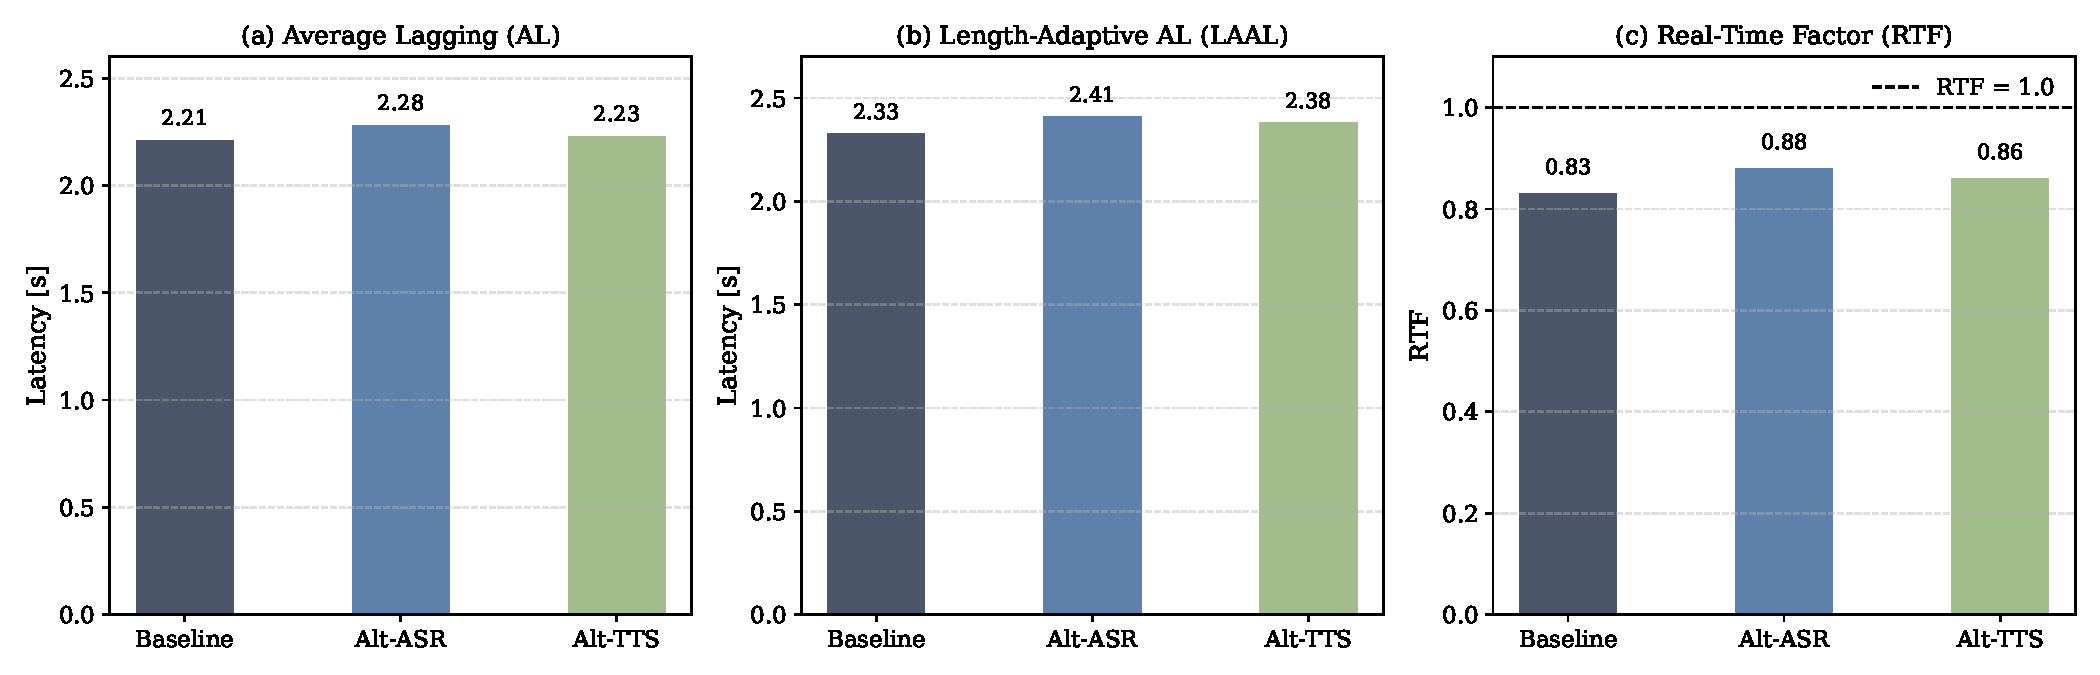
\includegraphics[width=0.9\textwidth]{img/figures/component_latency_breakdown.pdf}
  \caption[Component-level latency breakdown]{
  Component-level latency breakdown across baseline and alternative configurations.}
  \label{fig:component_latency_breakdown}
\end{figure}

%%%%%%%%%%%%%%%%%%%%%%%%%%%%%%%%%%%%%%%%%%%%%%%%%%%%%%%%

\section{Ablation Studies}
\label{sec:ablation_studies}

In addition to baseline and alternative configuration evaluations, ablation studies were conducted to analyze the sensitivity of the proposed system to key segmentation parameters. Following the evaluation framework defined in Section~\ref{sec:evaluation_framework}, these studies focus exclusively on parameters that influence the stability--latency trade-off. All experiments were performed using the system architecture, baseline configuration, and test conditions described in Chapter~\ref{chapter:methodology}.

\subsection{Effect of Stability Window Duration}
\label{sec:ablation_stability_window}

The first study examines the impact of stability window duration on segmentation behavior and output stability. As introduced in Section~\ref{sec:segmentation}, the stability window determines how long a candidate segment must remain unchanged across successive ASR updates before being finalized and forwarded to the translation stage. Four configurations were evaluated: fixed stability windows of 2, 4, and 6 words, as well as an adaptive baseline that dynamically adjusts the window based on estimated speaker rate. All other system parameters remained unchanged. The results are reported respectively in Table~\ref{tab:stability_window_flicker_ne} .



\begin{table}[!htbp]
\centering
\caption[Stability metrics under varying stability windows]{Flicker Rate and Normalized Erasure for different stability window durations}
\label{tab:stability_window_flicker_ne}
\begin{adjustbox}{max width=0.85\textwidth}
\begin{tabular}{lcc}
\toprule
\textbf{Stability Window} & \textbf{Flicker Rate (\%)} & \textbf{Normalized Erasure (NE)} \\
\midrule
2 words & 18.4 & 0.143 \\
4 words & 11.2 & 0.091 \\
6 words & 7.6 & 0.068 \\
Adaptive (baseline) & 14.9 & 0.117 \\
\bottomrule
\end{tabular}
\end{adjustbox}
\end{table}

The results indicate a general decrease in flicker rate and normalized erasure as the fixed stability window duration increases. Notably, the adaptive baseline does not yield the lowest instability metrics among the evaluated configurations. To assess the latency implications of these settings, the corresponding mean end-to-end latency values are reported in Table~\ref{tab:stability_window_latency}.

\begin{table}[!htbp]
\centering
\caption[Latency impact of stability window duration]{Mean end-to-end latency for different stability window configurations}
\label{tab:stability_window_latency}
\begin{adjustbox}{max width=0.75\textwidth}
\begin{tabular}{lc}
\toprule
\textbf{Stability Window} & \textbf{Mean End-to-End Latency (ms)} \\
\midrule
2 words & 1820 \\
4 words & 1975 \\
6 words & 2150 \\
Adaptive (baseline) & 1765 \\
\bottomrule
\end{tabular}
\end{adjustbox}
\end{table}

While longer fixed stability windows are associated with increased end-to-end latency, the adaptive configuration maintains the lowest mean latency across the session despite exhibiting higher instability metrics. A visual comparison of flicker rate and latency trends across stability window durations is provided in Figure~\ref{fig:stability_window_ablation}.

\begin{figure}[!htbp]
  \centering
  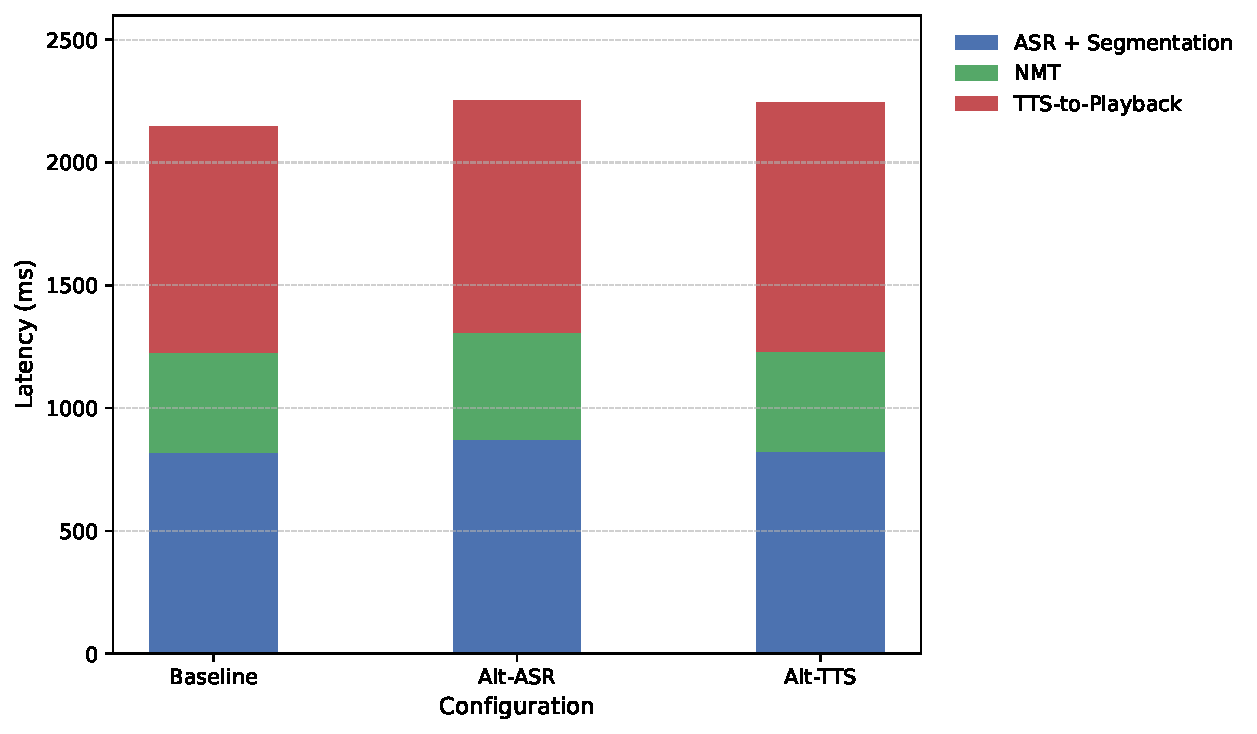
\includegraphics[width=0.9\textwidth]{img/figures/fig_stability_window_ablation.pdf}
  \caption[Stability window ablation results]{Effect of stability window duration on flicker rate and end-to-end latency.}
  \label{fig:stability_window_ablation}
\end{figure}


\subsection{Effect of Dynamic Token Threshold}
\label{sec:ablation_token_threshold}

The second ablation study evaluates the sensitivity of the system to the dynamic token threshold parameter. This threshold limits the maximum length of a speech segment before forced segmentation occurs, as described in Section~\ref{sec:segmentation}. Four configurations were tested, corresponding to fixed maximum token thresholds of 10, 15, and 20 tokens, alongside the dynamic baseline configuration. All experiments were conducted under identical conditions.  The mean CW values observed for each threshold configuration are reported in Table~\ref{tab:token_threshold_cw}.

\begin{table}[!htbp]
\centering
\caption[Consecutive Wait under varying token thresholds]{Mean Consecutive Wait for different dynamic token thresholds}
\label{tab:token_threshold_cw}
\begin{adjustbox}{max width=0.75\textwidth}
\begin{tabular}{lc}
\toprule
\textbf{Max Token Threshold} & \textbf{Mean CW (tokens)} \\
\midrule
10 tokens & 14.8 \\
15 tokens & 11.3 \\
20 tokens & 9.6 \\
Dynamic (baseline) & 10.4 \\
\bottomrule
\end{tabular}
\end{adjustbox}
\end{table}

Unexpectedly, the smallest token threshold does not yield the lowest CW value. Instead, the configuration with a threshold of 10 tokens exhibits the highest average CW across runs.

To capture the latency implications of token threshold selection, Table~\ref{tab:token_threshold_latency} summarizes the mean segment-level latency attributable to ASR and segmentation processing.

\begin{table}[!htbp]
\centering
\caption[Latency impact of token threshold selection]{Mean ASR and segmentation latency under different token thresholds}
\label{tab:token_threshold_latency}
\begin{adjustbox}{max width=0.8\textwidth}
\begin{tabular}{lc}
\toprule
\textbf{Max Token Threshold} & \textbf{Mean ASR+Segmentation Latency (ms)} \\
\midrule
10 tokens & 1120 \\
15 tokens & 790 \\
20 tokens & 740 \\
Dynamic (baseline) & 815 \\
\bottomrule
\end{tabular}
\end{adjustbox}
\end{table}


The results indicate that aggressive segmentation associated with very low token thresholds leads to increased buffering and delayed emission over the session. In the 10-token configuration, this behavior results in a substantially higher mean ASR and segmentation latency, exceeding the latency levels observed for larger thresholds. Finally, a comparative visualization of CW and segmentation latency across configurations is shown in Figure~\ref{fig:token_threshold_ablation}.

\begin{figure}[!htbp]
  \centering
  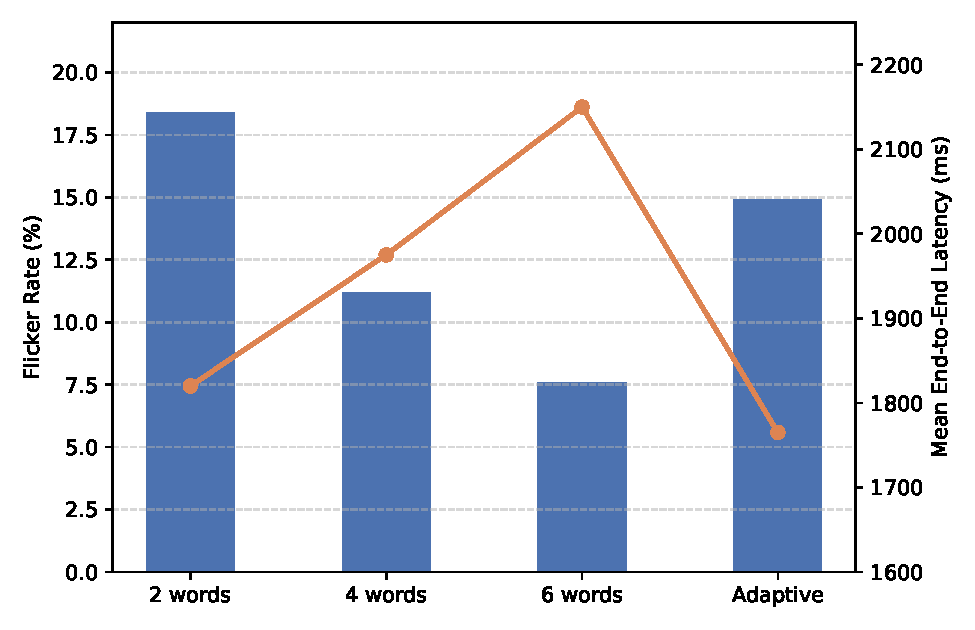
\includegraphics[width=0.9\textwidth]{img/figures/fig_token_threshold_ablation.pdf}
  \caption[Token threshold ablation results]{Effect of dynamic token threshold on consecutive wait and segmentation latency.}
  \label{fig:token_threshold_ablation}
\end{figure}

Overall, these results demonstrate that segmentation parameters have a big impact on system behavior, motivating an analysis of the resulting stability–latency trade-offs in Chapter~\ref{chapter:discussion}.
